\documentclass[a4paper,11pt,landscape,exos]{nsi} % COMPILE WITH DRAFT
\usepackage{hyperref}



\pagestyle{empty}
\setlength{\columnseprule}{0.5pt}
\setlength{\columnsep}{1cm}
\begin{document}

\begin{multicols}{2}
\classe{\premiere spe}
\titre{
\includegraphics[width=3cm]{CAN.png} Entrainement 6}
\maketitle

\begin{enumerate}[]
    \item  $9-9\times9$
	\item $25\,\%$ de $160$
	\item Écrire sous forme d'une fraction irréductible $\dfrac{1}{5}\times \dfrac{-5}{7}$.
	\item $\dfrac{3^{2}}{3^{4}}=3^{\ldots}$
	\item $1-\dfrac{1}{3}$ 
	\item Soit le script Python : 

\medskip
\medskip\hspace*{10mm}\fbox{\parbox{0.5\linewidth}{\setlength{\parskip}{.5cm} \texttt{def resultat(a) :}\newline \hspace*{7mm}\texttt{return (a**2-2*a)}}}\newline\medskip\\Que renvoie  $\texttt{resultat(-4)}$ ?
	\item $A$ et $B$ sont des événements indépendants tels que $P(A)=0{,}3$ et $P(B)=0{,}7$.
\\ $P(A\cap B)=\ldots$.
	\item La suite $(u_n)$ est géométrique telle que  $u_{2}= 28$ et $u_{3}= 7$.\\Sa raison $q$ est $\ldots$
	\item Quel est l'extremum sur $\mathbb{R}$ de  $x\longmapsto -3(x+4)^2+8$ ?  
	\item $\vec{u}\begin{pmatrix}5 \\4\end{pmatrix}$ et $\vec{v}\begin{pmatrix}10 \\ 8\end{pmatrix}$ ont la même direction. \\ 
    
    	$\square\;$ Vrai\qquad $\square\;$ Faux\qquad 
	\item Donner le nombre d'antécédent(s) de $-3$ par la fonction carré. 
	\item $225^2-224^2$ 
	\item Deux diminutions successives de  $40\,\%$ correspondent à une diminution globale de  $\ldots \,\%$.
	\item $\pc{A}{-3}{5}$ et $\pc{B}{2}{3}$\\
         Déterminer les coordonnées de $\vv{AB}$.\\[.5em]$\vc{AB}{\ldots}{\ldots}$
	\item $A$ et $B$ sont deux événements tels que :\\
	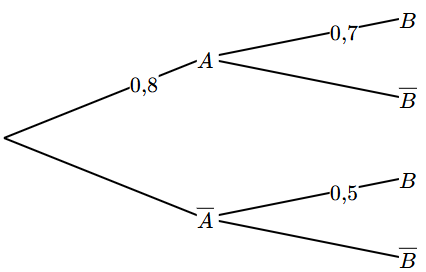
\includegraphics[width=5cm]{CAN6arbre.png}\\
    %\[\Proba[Arbre,Angle=40,Branche=3,Rayon=0.75,Incline=false]{A/$0.8$,$\overline{A}$/,B/$0.7$,$\overline{B}$/,B/$0.5$,$\overline{B}$/}\]
$P(B)=\ldots$ 
\end{enumerate}

\vfill\null

Score : \ldots\ldots / 15
\end{multicols}

\newpage

\begin{multicols}{2}
    \classe{\premiere spe}
\titre{
\includegraphics[width=3cm]{CAN.png} Corrigé 5}
\maketitle

\begin{enumerate}[]
\item $9-9\times9={\color[HTML]{f15929}\boldsymbol{-72}}$
\item $25\,\%$ de $160 = {\color[HTML]{f15929}\boldsymbol{40}}$\\ Prendre $25\,\%$  de $160$ revient à prendre le quart de $160$.\\
      Ainsi, $25\,\%$ de $160$ est égal à $160\div 4 =40$.
     
\item $\dfrac{1}{5}\times \dfrac{-5}{7}=-\dfrac{1{\color[HTML]{2563a5}\boldsymbol{\times5}} }{7{\color[HTML]{2563a5}\boldsymbol{\times5}}}={\color[HTML]{f15929}\boldsymbol{-\dfrac{1}{7}}}$
\item On utilise la formule $\dfrac{a^n}{a^p}=a^{n - p}$
        avec $a=3$,  $n=2$ et $p=4$.\\
        $\dfrac{3^{2}}{3^{4}}=3^{2-4}=3^{{\color[HTML]{f15929}\boldsymbol{-2}}}$
\item On a : \\$\begin{aligned}
      1+\dfrac{1}{3} &= \dfrac{1 \times 3}{3} - \dfrac{1}{3} \\
      &= \dfrac{3}{3} - \dfrac{1}{3}\\
      &  ={\color[HTML]{f15929}\boldsymbol{\dfrac{2}{3}}}
      \end{aligned}$
\item  L'algorithme renvoie $(-4)^2-2\times(-4)={\color[HTML]{f15929}\boldsymbol{24}}$.
\item  Comme $A$ et $B$ sont des événements indépendants,  $P(A\cap B)=P(A)\times  P(B)$.\\
Ainsi, \\
$\begin{aligned}
P(A\cap B)&=0{,}3 \times 0{,}7\\
P(A\cap B)&={\color[HTML]{f15929}\boldsymbol{0{,}21}}
\end{aligned}$
  
\item On passe de $u_{2}$ à $u_{3}$ en divisant par $4$, c'est-à-dire en multipliant par $\dfrac{1}{4}$.\\
    La raison de la suite est donc ${\color[HTML]{f15929}\boldsymbol{\dfrac{1}{4}}}$.
\item On reconnaît la forme canonique d'une fonction polynôme du second degré :\[f(x)=a(x-\alpha)^2+\beta\] où $\beta$ est l'extremum.\\
    L'extremum de $f$ est ${\color[HTML]{f15929}\boldsymbol{8}}$.
\item  
    
    	$\blacksquare\;$ Vrai\qquad $\square\;$ Faux\qquad Les vecteurs ont la même direction lorsqu'ils sont colinéaires.\\
    On a $\vec{v}=2\times \vec{u}$, donc les vecteurs ont la même direction. 
\item Comme $-3 < 0$, l'équation $x^2=-3$  n'a aucune solution. \\
    Ainsi, $-3$ a ${\color[HTML]{f15929}\boldsymbol{0}}$ antécédent par la fonction carré.
\item On utilise l'égalité remarquable $a^2-b^2=(a+b)(a-b)$ avec $a=225$ et $b=224$.\\
    $\begin{aligned}
    225^2-224^2&=(225+224)(225-224)\\
    &=449\times 1\\
    &={\color[HTML]{f15929}\boldsymbol{449}}
    \end{aligned}$
\item  Le coefficient multiplicateur  associé à une baisse de $40\,\%$ est $0{,}6$.\\
    Le coefficient multiplicateur global associé à ces deux diminutions est $0{,}6\times 0{,}6= 0{,}36$.\\
    On en déduit que le taux d'évolution globale est $0{,}36-1=-0{,}64$.\\
    La diminution globale est donc de ${\color[HTML]{f15929}\boldsymbol{64}} \,\%$.
\item $\vc{AB}{x_B-x_A}{y_B-y_A}$ donc $\vc{AB}{2-(-3)}{3-5}$.\\
         Ainsi, $\vc{AB}{\color[HTML]{f15929}{5}}{\color[HTML]{f15929}{-2}}$. 
\item On utilise la formule des probabilités totales pour calculer $P(B)$ :\\
              $\begin{aligned}
              P(B)&=P(A\cap B)+P(\bar{A}\cap B)\\
              &=0{,}8\times 0{,}7+0{,}2\times 0{,}5\\
    &={\color[HTML]{f15929}\boldsymbol{0{,}66}}
              \end{aligned}$
   
      \vfill\null
      \columnbreak
\end{enumerate}
$\quad$\\
\end{multicols}

\end{document}

